\documentclass[a4paper]{report}

\usepackage[margin=3.0cm]{geometry}
\usepackage{amsmath}
\usepackage[pdftex]{graphicx}
%\usepackage{graphics}
\usepackage{subfig}



\title{HPMPC reference guide}
\author{Gianluca Frison}



\begin{document}

\maketitle
\tableofcontents

%%%%%%%%%%%%%%%%%%%%%%%%%%%%%%%%
\chapter{Introduction}
%%%%%%%%%%%%%%%%%%%%%%%%%%%%%%%%

HPMPC -- A library for High-Performance implementation of solvers for MPC.

HPMPC has been developed with the aim of providing extremely fast building blocks to implement algorithms for Model Predictive Control (MPC). 
This has been achieved by carefully implementing the linear algebra routines using high-performance computing techniques with a focus on small-medium scale problems, typical of MPC applications.

The current version of the library contains a Mehrotra predictor-corrector Interior-Point Method (IPM) solver for the linear MPC problem with box and general affine constraints, and a Riccati-based solver for the unconstrained MPC problem, that is used as a routine in the IPM.
A simple API is provided for these solvers, while lower level interfaces provide access to kernels, linear-algebra routines and MPC solvers.
The library is self-contained, not requiring any other library beside the standard C library.

The code is highly-optimized for a number of common architectures, plus a reference version in plain C code (C99 standard).
The code has been developed on Linux machines and tested also on MAC machines. 
The code is intended to be compiled using {\tt gcc} as a compiler (the code for some architecture makes use of extended asm inline assembly); it can be compiled using {\tt clang} as well, while it may need some hacking to work with other compilers.
In any case, the time-critical routines have been carefully implemented in assembly exploiting architecture-specific features, so there would be no practical advantage in compiling the code with more performing (e.g. commercial) compilers.

The library is released under the LGPL version 3 licence, and it can be used as a basis for the development of higher-level solvers for MPC or other applications requiring extremely fast solvers for small-medium scale problems.



%%%%%%%%%%%%%%%%%%%%%%%%%%%%%%%%
\chapter{Problems definition}
%%%%%%%%%%%%%%%%%%%%%%%%%%%%%%%%

In this chapter the unconstrained and constrained MPC problems are presented.

%%%%%%%%%%%%%%%%
\section{Unconstrained MPC Problem}
%%%%%%%%%%%%%%%%

The unconstrained MPC problem is the equality constrained quadratic program
\begin{equation}
\begin{aligned}
\min_{u_n,x_n} &&& \phi = \sum_{n=0}^{N-1} \varphi_n(x_n,u_n) + \varphi_N(x_N) \\
s.t. &&& x_{n+1} = A_nx_n+B_nu_n+b_n \\
&&& x_0 = \hat x_0
\end{aligned}
\label{lqcp}
\end{equation}
where $n\in\{0,1,\dots,N-1\}$ and
\begin{equation}
\begin{aligned}
\varphi_n(x_n,u_n) &= \begin{bmatrix} u_n \\ x_n \\ 1 \end{bmatrix}^T \begin{bmatrix} R_n&S_n&r_n \\ S_n^T&Q_n&q_n \\ r_n^T&q_n^T& \rho_n \end{bmatrix} \begin{bmatrix} u_n \\ x_n \\ 1 \end{bmatrix}  = \mathcal{X}^T_n\mathcal{Q}_n\mathcal{X}_n \\
\varphi_N(x_N) &= \begin{bmatrix} u_N \\ x_N \\ 1 \end{bmatrix}^T \begin{bmatrix} 0&0&0 \\ 0&Q_N&q_N \\ 0&q_N^T&\rho_N \end{bmatrix} \begin{bmatrix} u_N \\ x_N \\ 1 \end{bmatrix} = \mathcal{X}^T_N\mathcal{Q}_N\mathcal{X}_N\\ 
\end{aligned}
\label{eq:cf_mpc}
\end{equation}
All matrices in this formulation can in general be dense and time variant. 
The matrices $\mathcal Q_n$ have to be symmetric and positive semi-definite, while the $R_n$ matrices have to be symmetric and strictly positive definite.

%%%%%%%%%%%%%%%%
\section{Linear MPC problem}
%%%%%%%%%%%%%%%%

The linear MPC problem with box and general polytopic constraints is the quadratic program
\begin{equation}
\begin{aligned}
\min_{u_n,x_n} &&& \phi = \sum_{n=0}^{N-1} \varphi_n(x_n,u_n) + \varphi_N(x_N) \\
s.t. &&& x_{n+1} = A_nx_n+B_nu_n+b_n \\
&&& x_0 = \hat x_0 \\
&&& u_n^l \leq u_n\leq u_n^u \\
&&& x_n^l \leq x_n\leq x_n^u \\
&&& d_n^l \leq C_n x_n + D_n u_n \leq d_n^u \\
&&& d_N^l \leq C_N x_n \leq d_N^u
\end{aligned}
\label{eq:lmpc}
\end{equation}
where $n\in\{0,1,\dots,N-1\}$, $\varphi_n(x_n,u_n)$ and $\varphi_N(x_N)$ are defined as in (\ref{eq:cf_mpc}). Again, all matrices can in general be dense and time variant.



%%%%%%%%%%%%%%%%%%%%%%%%%%%%%%%%
\chapter{Compilation and installation of the library}
%%%%%%%%%%%%%%%%%%%%%%%%%%%%%%%%

The code has been developed on Linux machines, using the {\tt gcc} compiler.
It has been also tested on MAC machines using the {\tt clang} compiler.
The library is mainly written in C code, with time-critical parts (kernels) written using intrinsics or extended asm inline assembly: from here the need for the {\tt gcc} or {\tt clang} compilers.

Time-critical routines are carefully optimized by hand for a number of architectures, using assembly to explicitly exploit e.g. the number of registers and SIMD instruction sets specific to each architecture.

%\section{Complilation}

%As already said, the code is expected to be compiled using {\tt gcc}, and is self-contained, depending only on the standard library.
The {\tt gcc} compiler is found already installed on most Linux distributions.

Redarding utilities, {\tt make} is used to automate the compilation of the code, and {\tt ar} to build the static library: both of them are found installed on all Linux distributions.
Alternatively, the library can be built using {\tt CMake}.

%%%%%%%%%%%%%%%%
\section{Target architectures}
%%%%%%%%%%%%%%%%

Once the code has been downloaded, the first step is the editing of the configuration file {\tt Makefile.rule}.
In general, the only part that needs to be edited is the {\tt TARGET}, used to choose architeture-specific code and flags.
In the following, the abbreviation ISA stands for Instruciton Set Architecture.

Currently supported targets are
\begin{description}

\item[X64\_AVX2] this a recent x86\_64 processor supporting AVX2 and FMA3 ISAs (e.g. Intel Haswell, Intel Broadwell or Intel Skylake micro-architectures). 
The 64-bit version of the OS is required. 
At the moment, these micro-architectures are supported, but only the double-precision version of the library if fully-optimized.

\item[X64\_AVX] this is a x86\_64 processor supporting the AVX ISA (e.g. Intel Sandy Bridge and Intel Ivy Bridge; AMD Bulldozer or more recent micro-architectures). 
The 64-bit version of the OS is required.

\item[X64\_SSE3] this is a x86\_64 processor supporting the SSE3 ISA (e.g. Intel Pentium 4 Prescott, Intel Core and Intel Nehalem; AMD Athlon 64 revision E or more recent micro-architectures). 
The 64-bit version of the OS is required. 
The code is not fully optimized yet.

\item[CORTEX\_A57] this is a processor implementing the ARMv8A architecture with VFPv4 and NEONv2 ISAs, code optimized for ARM Cortex A57.
At the moment the architecture is supported using reference code, and only the {\tt dgemm} and {\tt sgemm} routines are optimized.

\item[CORTEX\_A15] this is a processor implementing the ARMv7A architecture with VFPv4 and NEONv2 ISAs, code optimized for ARM Cortex A15.

\item[CORTEX\_A9] this is a processor implementing the ARMv7A architecture with VFPv3 and NEON ISAs, code optimized for ARM Cortex A9.

\item[CORTEX\_A7] this is a processor implementing the ARMv7A architecture with VFPv4 and NEONv2 ISAs, code optimized for ARM Cortex A7.

\item[C99\_4X4] this version is written entirely in C code and works with all machines, even if performing worse that machine-specific code. 
The code works better on a machine with at least 32 scalar FP registers.

\end{description}
More architectures are supported in the older version 0.1 of the library, that can still be downloaded from github.

The supported ISAs can be easily found by googling the processor name, or (on Linux machines) by typing
\begin{verbatim}
less \proc\cpuinfo
\end{verbatim}
on a terminal, and looking among the flags. 
In any case, even if the code is compiled for the wrong architecutre, an {\tt Illegal instruction} error will be raised at run time, so this can be immediately discovered running a test problem.

%%%%%%%%%%%%%%%%
\section{Compilation and installation process}
%%%%%%%%%%%%%%%%

Once the architecture has been chosen, the static library can be build by typing
\begin{verbatim}
make static_library
\end{verbatim}
on a terminal. The dynamic library can be build by typing
\begin{verbatim}
make shared_library
\end{verbatim}
on a terminal.

The macro {\tt PREFIX} in the configuration file {\tt Makefile.rule} contains the installation directory (the default one is {\tt /opt}).
The static library and the headers can be installed by typing
\begin{verbatim}
sudo make install_static
\end{verbatim}
on a terminal. The dynamic library and the headers can be installed by typing
\begin{verbatim}
sudo make install_shared
\end{verbatim}
on a terminal.

The libraries and the headers can be uninstalled by typing
\begin{verbatim}
sudo make uninstall
\end{verbatim}
on a terminal.



%%%%%%%%%%%%%%%%%%%%%%%%%%%%%%%%
\chapter{Running test problems}
%%%%%%%%%%%%%%%%%%%%%%%%%%%%%%%%

%%%%%%%%%%%%%%%%
\section{Running Octave test problems}
%%%%%%%%%%%%%%%%

A number of Octave test problems is vailable in the folder {\tt interfaces/octave}.

A {\tt mex} interface is used as a wrapper around the high-level API for the solvers.
Octave test problems call the {\tt mex} wrappers.

%%%%%%%%
\subsection{Constrained MPC problem example}
%%%%%%%%

Here the Octave interface of the IPM solver is used to solve the constrained linear MPC problem.
The test problem is {\tt interfaces/octave/test\_ip\_hard.m}.

The mex wrapper to the IPM solver is contained in the file {\tt interfaces/octave/HPMPC\_ip\_hard.c}.
The interface to solve hard-constrained linear MPC problems looks like
\begin{verbatim}
HPMPC_ip_hard(kk, k_max, mu0, tol, N, nx, nu, nb, ng, ngN, time_invariant, 
A, B, b, Q, QN, R, S, q, qN, r, lb, ub, C, D, lg, ug, CN, lgN, ugN, x, u, 
infos, compute_res, inf_norm_res, compute_mult, mult_pi, mult_lam, mult_t);
\end{verbatim}
where
\begin{description}

\item[\tt kk] Output: the number of iterations for the IPM to converge.

\item[\tt k\_max] Input: maximum number of iterations in the IPM.

\item[\tt mu0] Input: initial value of the parameter $\mu$ in the IPM.
If equal or smaller than 0, it is fixed in the IPM as the largest absolute value of the elements of the cost function matrices and vectors.

\item[\tt tol] Input: tolerance on the duality measure for convergence.

\item[\tt N] Input: horizon lenght, where 0 is the fist stage, 1 to N-1 are the middle stages and N is the last stage.

\item[\tt nx] Input: number of states per stage.

\item[\tt nu] Input: number of inputs per stage.

\item[\tt nb] Input: number of box constraints per stage, meaning that the first {\tt nb} element of the variables vector at each stage are bounded, where the variables vector at the generic stage $n$ is $v_n = \begin{bmatrix} u_n^T & x_n^T \end{bmatrix}^T$.

\item[\tt ng] Input: number of general constraints on stages 0 to N-1.

\item[\tt ngN] Input: number of general constraints at the last stage N.

\item[\tt time\_invariant] Input: flag to choose between time-invariant (1) and time-variant (0) interfaces.

\item[\tt A] Input: corresponds to the $A_n$ matrix in (\ref{eq:lmpc}).
If {\tt time\_invariant} is 1, then {\tt A} is a $n_x\times n_x$ matrix; if {\tt time\_invariant} is 0, then {\tt A} is a $n_x\times Nn_x$ matrix, corresponding to $\begin{bmatrix} A_0 & A_1 & \dots & A_{N-1} \end{bmatrix}$.

\item[\tt B] Input: corresponds to the $B_n$ matrix in (\ref{eq:lmpc}).
If {\tt time\_invariant} is 1, then {\tt B} is a $n_x\times n_u$ matrix; if {\tt time\_invariant} is 0, then {\tt B} is a $n_x\times Nn_u$ matrix, corresponding to $\begin{bmatrix} B_0 & B_1 & \dots & B_{N-1} \end{bmatrix}$.
\item[\tt b] Input: corresponds to the $b_n$ vector in (\ref{eq:lmpc}).
If {\tt time\_invariant} is 1, then {\tt b} is a $n_x\times 1$ matrix; if {\tt time\_invariant} is 0, then {\tt b} is a $n_x\times N$ matrix, corresponding to $\begin{bmatrix} b_0 & b_1 & \dots & b_{N-1} \end{bmatrix}$.
\item[\tt Q] Input: corresponds to the $Q_n$ matrix in (\ref{eq:cf_mpc}).
If {\tt time\_invariant} is 1, then {\tt Q} is a $n_x\times n_x$ matrix; if {\tt time\_invariant} is 0, then {\tt Q} is a $n_x\times Nn_x$ matrix, corresponding to $\begin{bmatrix} Q_0 & Q_1 & \dots & Q_{N-1} \end{bmatrix}$.

\item[\tt QN] Input: corresponds to the $Q_N$ matrix in (\ref{eq:cf_mpc}).
{\tt QN} is a $n_x\times n_x$ matrix.

\item[\tt R] Input: corresponds to the $R_n$ matrix in (\ref{eq:cf_mpc}).
If {\tt time\_invariant} is 1, then {\tt R} is a $n_u\times n_u$ matrix; if {\tt time\_invariant} is 0, then {\tt R} is a $n_u\times Nn_u$ matrix, corresponding to $\begin{bmatrix} R_0 & R_1 & \dots & R_{N-1} \end{bmatrix}$.

\item[\tt S] Input: corresponds to the $S_n$ matrix in (\ref{eq:cf_mpc}).
If {\tt time\_invariant} is 1, then {\tt S} is a $n_u\times n_x$ matrix; if {\tt time\_invariant} is 0, then {\tt S} is a $n_u\times Nn_x$ matrix, corresponding to $\begin{bmatrix} S_0 & S_1 & \dots & S_{N-1} \end{bmatrix}$.

\item[\tt q] Input: corresponds to the $q_n$ vector in (\ref{eq:cf_mpc}).
If {\tt time\_invariant} is 1, then {\tt q} is a $n_x\times 1$ matrix; if {\tt time\_invariant} is 0, then {\tt q} is a $n_x\times N$ matrix, corresponding to $\begin{bmatrix} q_0 & q_1 & \dots & q_{N-1} \end{bmatrix}$.

\item[\tt qN] Input: corresponds to the $q_N$ vector in (\ref{eq:cf_mpc}).
{\tt qN} is a $n_x\times 1$ matrix.

\item[\tt r] Input: corresponds to the $r_n$ vector in (\ref{eq:cf_mpc}).
If {\tt time\_invariant} is 1, then {\tt r} is a $n_u\times 1$ matrix; if {\tt time\_invariant} is 0, then {\tt r} is a $n_u\times N$ matrix, corresponding to $\begin{bmatrix} r_0 & r_1 & \dots & r_{N-1} \end{bmatrix}$.

\item[\tt lb] Input: corresponds to the $\begin{bmatrix} (u_n^l)^T & (x_n^l)^T \end{bmatrix}^T$ vector in (\ref{eq:cf_mpc}).
If {\tt time\_invariant} is 1, then {\tt lb} is a $n_b\times 1$ matrix; if {\tt time\_invariant} is 0, then {\tt lb} is a $n_b\times (N+1)$ matrix, corresponding to $\begin{bmatrix} u^l_0 & u^l_1 & \dots & u^l_{N-1} & * \\ * & x^l_1 & \dots & x^l_{N-1} & x^l_N \end{bmatrix}$.

\item[\tt ub] Input: corresponds to the $\begin{bmatrix} (u_n^u)^T & (x_n^u)^T \end{bmatrix}^T$ vector in (\ref{eq:cf_mpc}).
If {\tt time\_invariant} is 1, then {\tt ub} is a $n_b\times 1$ matrix; if {\tt time\_invariant} is 0, then {\tt ub} is a $n_b\times (N+1)$ matrix, corresponding to $\begin{bmatrix} u^u_0 & u^u_1 & \dots & u^u_{N-1} & * \\ * & x^u_1 & \dots & x^u_{N-1} & x^u_N \end{bmatrix}$.

\item[\tt C] Input: corresponds to the $C_n$ matrix in (\ref{eq:lmpc}).
If {\tt time\_invariant} is 1, then {\tt C} is a $n_g\times n_x$ matrix; if {\tt time\_invariant} is 0, then {\tt C} is a $n_g\times Nn_x$ matrix, corresponding to $\begin{bmatrix} C_0 & C_1 & \dots & C_{N-1} \end{bmatrix}$.

\item[\tt D] Input: corresponds to the $D_n$ matrix in (\ref{eq:lmpc}).
If {\tt time\_invariant} is 1, then {\tt D} is a $n_g\times n_u$ matrix; if {\tt time\_invariant} is 0, then {\tt D} is a $n_g\times Nn_u$ matrix, corresponding to $\begin{bmatrix} D_0 & D_1 & \dots & D_{N-1} \end{bmatrix}$.

\item[\tt lg] Input: corresponds to the $d^l_n$ matrix in (\ref{eq:lmpc}).
If {\tt time\_invariant} is 1, then {\tt lg} is a $n_g\times 1$ matrix; if {\tt time\_invariant} is 0, then {\tt lg} is a $n_g\times N$ matrix, corresponding to $\begin{bmatrix} d^l_0 & d^l_1 & \dots & d^l_{N-1} \end{bmatrix}$.

\item[\tt ug] Input: corresponds to the $d^u_n$ matrix in (\ref{eq:lmpc}).
If {\tt time\_invariant} is 1, then {\tt ug} is a $n_g\times 1$ matrix; if {\tt time\_invariant} is 0, then {\tt ug} is a $n_g\times N$ matrix, corresponding to $\begin{bmatrix} d^u_0 & d^u_1 & \dots & d^u_{N-1} \end{bmatrix}$.

\item[\tt CN] Input: corresponds to the $C_N$ matrix in (\ref{eq:lmpc}).
{\tt CN} is a $n_{gN}\times n_x$ matrix.

\item[\tt lgN] Input: corresponds to the $d^l_N$ matrix in (\ref{eq:lmpc}).
{\tt lgN} is a $n_{gN}\times 1$ matrix.

\item[\tt ugN] Input: corresponds to the $d^u_N$ matrix in (\ref{eq:lmpc}).
{\tt ugN} is a $n_{gN}\times 1$ matrix.

\item[\tt x] It is a matrix of size $n_x \times N+1$.
Input: the first column correspond to $\hat x_0$ (\ref{eq:lmpc}).
Output: the columns from 2 to N+1 return the state vector at the solution, corresponding to stages 1 to N respectively.

\item[\tt u] It is a matrix of size $n_u \times N$.
Output: the columns from 1 to N return the input at the solution, corresponding to stages 1 to N respectively.

\item[\tt infos] It is a matrix of size $kk \times 5$.
Output: informations about the IPM covergence at each IPM iteration: $\sigma$, $\alpha_{\rm aff}$, $\mu_{\rm aff}$, $\alpha$, $\mu$.

\item[\tt compute\_res] Input: flags that enables (1) or disables (0) the comutation of the residuals.

\item[\tt inf\_norm\_res] It is a vector of size 4.
Output: it returns $\begin{bmatrix} ||r_q||_\infty & ||r_b||_\infty & ||r_d||_\infty & \mu \end{bmatrix}^T$.

\item[\tt compute\_mult] Input: flags that enables (1) or disables (0) the comutation of the Lagrangian multipliers.

\item[\tt mult\_pi] Matrix of size $n_x \times N+1$.
Output: it returns the Lagrangian multipliers of the equality constraints.

\item[\tt mult\_lam] Vector of size $2(n_b+n_g)N + 2(n_b+n_{gN})$.
Output: it returns the Lagrangian multipliers of the inequality constraints.

\item[\tt mult\_t] Vector of size $2(n_b+n_g)N + 2(n_b+n_{gN})$.
Output: it returns the slack variables associated with Lagrangian multipliers of the inequality constraints.

\end{description}

%TODO add a flag to make the interface handling time-invariant problems.

%%%%
\subsubsection{Time-invariant case}
%%%%

The test problem is the mass-spring system, that has been widely used to test linear MPC solvers thanks to its scalability properties.

The problem size is $N=30$, $n_x=8$, $n_u=3$.
Therefore there are 4 masses, and a force acts on the the first 3 of them.
Each mass is equal to 1 Kg, and the constant of each spring is equal to 1 N/m.

The forces are bounded between $-0.5$ and $0.5$.
The position of the masses is bounded between $-4.0$ and $4.0$.
The velocity of the masses is not constrainted.
A terminal constraint imposes that the position and the velocity of all masses must be equal to 0 (i.e. the masses must be at resting position at stage N).
Since the bounds are time-invariant, the terminal constraints must be handled as general polytopic constraints at the last stage N.

Therefore, the number of bounds is $n_b=n_u+\tfrac{n_x} 2 = 7$.
Since only the first $\tfrac{n_x} 2$ states are bounded, the states are ordered such that the first $\tfrac{n_x} 2$ states corresponds to the masses position.
The number of general polytopic constraints at stages 0 to N-1 is $n_g = 0$.
The number of general polytopic constraints at the last stage $N$ is $n_{gN} = 8$.

The cost function matrices and vectors are initialized as: $Q=I$, $QN=I$, $R=2I$, $S=0$, $q=0$, $qN=0$, $r=0$. 

The initial state is 

About the choice of the IPM parameters, the maximum number of iterations is fixed to 20.
The tolerance in the duality measure is fixed to $10^{-8}$.
Since the largest absolute value of the elements in the cost function expression is 2, it holds $\mu_0=2$.
Both residuals and Lagrangian multipliers are computed.

The code is runned on a Linux machine with processor Intel core i7 3520M, and 8 GB of DDR3 RAM in dual-channel configuration, running at 1600 MHz (maximum bandwidth of 25.6 GB/s).
The HPMPC library is compiled for the AVX target.

The IPM solver returns after 8 iterations, and the solution time averaged over 1000 calls to the IPM solver is $3.14\cdot 10^{-4}$ seconds.

The {\tt infos} about the IPM iterations are summarized in Table \ref{tab:infos}
\begin{table}
\centering
\caption{Content of the {\tt infors} matrix.}
\label{tab:infos}
\begin{tabular}{c|ccccc}
iteration & $\sigma$ & $\alpha_{\rm aff}$ & $\mu_{\rm aff}$ & $\alpha$ & $\mu$ \\ 
\hline
1 &   $2.7514\cdot 10^{-01}$ &  $3.2839\cdot 10^{-01}$ &  $1.3008\cdot 10^{+00}$ &  $3.9179\cdot 10^{-01}$ &  $1.5862\cdot 10^{+00}$ \\
2 &   $7.7808\cdot 10^{-02}$ &  $5.4011\cdot 10^{-01}$ &  $6.7718\cdot 10^{-01}$ &  $7.1498\cdot 10^{-01}$ &  $6.2662\cdot 10^{-01}$ \\
3 &   $4.3610\cdot 10^{-03}$ &  $8.3084\cdot 10^{-01}$ &  $1.0238\cdot 10^{-01}$ &  $9.1943\cdot 10^{-01}$ &  $6.2629\cdot 10^{-02}$ \\
4 &   $2.2303\cdot 10^{-02}$ &  $7.3060\cdot 10^{-01}$ &  $1.7629\cdot 10^{-02}$ &  $8.8868\cdot 10^{-01}$ &  $8.7287\cdot 10^{-03}$ \\
5 &   $8.6078\cdot 10^{-03}$ &  $8.1046\cdot 10^{-01}$ &  $1.7889\cdot 10^{-03}$ &  $9.3176\cdot 10^{-01}$ &  $7.4587\cdot 10^{-04}$ \\
6 &   $1.8652\cdot 10^{-03}$ &  $8.9358\cdot 10^{-01}$ &  $9.1813\cdot 10^{-05}$ &  $9.8345\cdot 10^{-01}$ &  $2.0746\cdot 10^{-05}$ \\
7 &   $3.1456\cdot 10^{-05}$ &  $9.8589\cdot 10^{-01}$ &  $6.5489\cdot 10^{-07}$ &  $9.9763\cdot 10^{-01}$ &  $1.9884\cdot 10^{-07}$ \\
8 &   $3.7490\cdot 10^{-07}$ &  $9.9926\cdot 10^{-01}$ &  $1.4338\cdot 10^{-09}$ &  $1.0000\cdot 10^{+00}$ &  $9.9658\cdot 10^{-10}$ \\
\end{tabular}
\end{table}

The absolute value of the residuals is
\begin{equation*}
\begin{bmatrix} ||r_q||_\infty \\ ||r_b||_\infty \\ ||r_d||_\infty \\ \mu \end{bmatrix} = \begin{bmatrix} 1.8806\cdot 10^{-06} \\ 3.0816\cdot 10^{-10} \\ 1.0004\cdot 10^{-11} \\ 9.9658\cdot 10^{-10} \end{bmatrix}
\end{equation*}

\begin{figure}%[!t]
\centering
\subfloat[States]{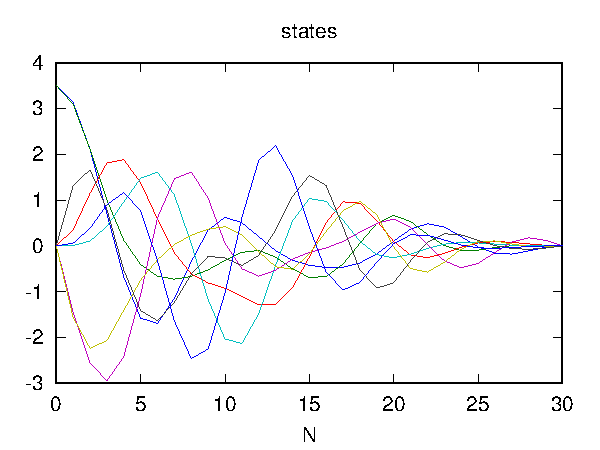
\includegraphics[width=0.5\linewidth]{states.pdf} \label{fig:sol:states}} %\\
\subfloat[Inputs]{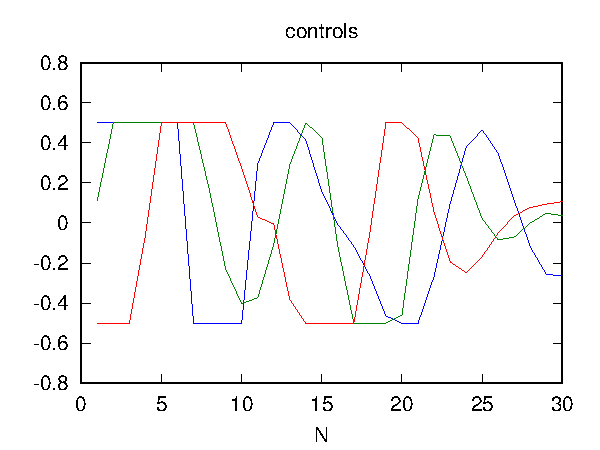
\includegraphics[width=0.5\linewidth]{inputs.pdf} \label{fig:sol:input}} \\
\caption{Solution.}
\label{fig:sol}
\end{figure}


%%%%
\subsubsection{Time-variant case}
%%%%

The time-invariant interface is more general than the time-invariant interface, and therefore it can handle the time-invariant case as well.
The drawback is that it needs to pack a different matrix at each stage, since all matrices and vectors can potentially be time-variant.

The matrix {\tt A} is built using the {\tt repmat} command in Octave, as
\begin{verbatim}
A = repmat(A0, 1, N);
\end{verbatim}
where {\tt A0} corresponds to the {\tt A} matrix in the time-invariant case.

Similarly are built the other state space and cost function matrices and vectors.

The returned results are identical to the time-invariant case.


%%%%%%%%%%%%%%%%
\section{Running C test problems}
%%%%%%%%%%%%%%%%

A number of test problems is available in the folder {\tt test\_problems}, and it is possible to choose between them by editing the file {\tt test\_problems/Makefile}.
Notice that test problems are not part of the library.
The chosen test problem is compiled by typing
\begin{verbatim}
make test_problem
\end{verbatim}
on a terminal opened on the main HPMPC folder, and it is run by typing
\begin{verbatim}
make run 
\end{verbatim}
on a terminal opened on the main HPMPC folder.



%%%%%%%%%%%%%%%%%%%%%%%%%%%%%%%%
\chapter{High-level API}
%%%%%%%%%%%%%%%%%%%%%%%%%%%%%%%%

In this chapter the high-level API is presented. 
It is intended to give access to the higher level routines in the library, namely the Riccati solver for the unconstrained problem (\ref{lqcp}), and the IPM solver for the MPC problem (\ref{eq:lmpc}).

For performance purposes, internally the library makes use of a packed matrix format, and routines are provided to convert to and from this packed format and standard column- and row-major orders.

In this high-level API, all matrices are passed using standard column- or row-major orders, and wrappers take care of the conversions into the panel-major order used internally by all solvers.
For the best performance, users may consider to skip the wrappers and directly call the underlying solvers (low-level API).

%%%%%%%%
\subsection{Constrained MPC problem example}
%%%%%%%%

The wrapper to the IPM solver is contained in the files {\tt interfaces/c/fortran\_oder\_interface.c} (assuming matrices to be passed in column-major order) and {\tt interfaces/c/c\_order\_interface.c} (assuming matrices to be passed in row-major order).
In the file {\tt interfaces/c/c\_interface\_work\_space.c} there are functions returing the amount of memory to be allocated (either dynamically or statically) and passes to the solvers.
No memory allocation takes place in the solvers.

The interface assuming the matrices to be passed in column-major order (the one assuming the matrices to be passed in row-major order) is
\begin{verbatim}
int fortran_order_d_ip_ocp_hard_tv( 
    int *kk, int k_max, double mu0, double mu_tol,
    int N, int *nx, int *nu, int *nb, int *ng,
    int warm_start,
    double **A, double **B, double **b, 
    double **Q, double **S, double **R, double **q, double **r, 
    double **lb, double **ub,
    double **C, double **D, double **lg, double **ug,
    double **x, double **u, double **pi, double **lam, double **t,
    double *inf_norm_res,
    void *work0, 
    double *stat)
\end{verbatim}
where
\begin{description}

\item[\tt int *kk] Output: point to int, returing the number of performed IPM iterations.

\item[\tt int k\_max] Input: int fixing the maximum number of IPM iterations.

\item[\tt double mu0] Input: initial value of the duality measure, used in the initialization of the slack variables and of the Lagrangian multipliers of the inequality constraints.

\item[\tt double mu\_tol] Input: minimum value of the duality measure to return from the IPM before the maximum number of iterations is reached.

\item[\tt int N] Input: control horizon length in the MPC problem.

\item[\tt int *nx] Input: array of length $N+1$, where {\tt nx[i]} is the number of states at stage $i$.

\item[\tt int *nu] Input: array of length $N+1$, where {\tt nu[i]} is the number of controls at stage $i$, and $nu[N]=0$.

\item[\tt int *nb] Input: array of length $N+1$, where {\tt nb[i]} is the number of two-sided box constraints at stage $i$.

\item[\tt int *ng] Input: array of length $N+1$, where {\tt ng[i]} is the number of two-sided general affine constraints at stage $i$.

\end{description}




%%%%%%%%%%%%%%%%%%%%%%%%%%%%%%%%
\chapter{References}
%%%%%%%%%%%%%%%%%%%%%%%%%%%%%%%%

The HPMPC library is the result of a long research path that led to a novel way to implement solvers for MPC, specially tailored to small-medium scale problems.
The library has undergone several revisions before being published, and some of the steps along this research path are documented in the following papers.
\begin{itemize}
\item G. Frison, H.H.B. S{\o}rensen, B. Dammann, J.B. J{\o}rgensen, \emph{ High-Performance Small-Scale Solvers for Linear Model Predictive Control}, in proceedings of 13th European Control Conference, Strasbourg (France), 2014.
\item G. Frison, L.E. Sokoler, J.B. J{\o}rgensen, \emph{A Family of High-Performance Solvers for Linear Model Predictive Control}, in proceedings of 19th IFAC World Congress, Cape Town (South Africa), 2014.
\item G. Frison, D.K.M. Kufualor, L. Imsland, J.B. J{\o}rgensen, \emph{Efficient Implementation of Solvers for Linear Model Predictive Control on Embedded Devices}, in proceedings of IEEE Multi-conference on Systems and Control, Antibes (France), 2014.
\item G. Frison, J.B. J{\o}rgensen, \emph{MPC Related Computational Capabilities of ARMv7A Processors}, in proceedings of 14th European Control Conference, Linz (Austria), 2015.
\end{itemize}


\end{document}
